\documentclass[conference]{IEEEtran}
\IEEEoverridecommandlockouts
\usepackage{cite}
\usepackage{amsmath,amssymb,amsfonts}
\usepackage{graphicx}
\usepackage{textcomp}
\usepackage{xcolor}
\usepackage{booktabs}
\def\BibTeX{{\rm B\kern-.05em{\sc i\kern-.025em b}\kern-.08em
    T\kern-.1667em\lower.7ex\hbox{E}\kern-.125emX}}
\begin{document}

\title{Auto-Echo: Formative Draft Dissertation\\
{\large Automated Discovery of Memory Hierarchy Latency Patterns from User-Space}
}

\author{\IEEEauthorblockN{Harsh Raj Singh}
\IEEEauthorblockA{\textit{MSc Advanced Computer Science} \\
\textit{Queen Mary University of London}\\
London, United Kingdom \\
ec25303@qmul.ac.uk}
}

\maketitle

\begin{abstract}
The memory hierarchy of modern computing architectures is increasingly complex, sparsely documented, and abstracted away from user-space applications. This limits the ability of software engineers to optimise performance-critical applications. This research introduces Auto-Echo, a cross-platform framework designed to empirically discover a machine's memory hierarchy (L1, L2, L3 caches, and DRAM) purely from user-space, without requiring administrative privileges. By bridging low-level systems programming with unsupervised machine learning, Auto-Echo attempts to autonomously classify hardware boundaries. This paper details the initial methodology---a randomised-access C probe combined with K-Means clustering---and critically analyses the empirical results. Testing on Apple Silicon revealed three barriers: coarse timer quantisation, the absence of a user-space cache-flush primitive on ARM, and a measurement-design flaw in which each timed read was preceded by a write to the same address, guaranteeing an L1 hit by construction. These findings provide a clear roadmap for the final submission, motivating a pointer-chasing working-set-size methodology with batch-amortised timing and change-point detection.
\end{abstract}

\begin{IEEEkeywords}
memory hierarchy, cache echolocation, unsupervised machine learning, K-Means, change-point detection
\end{IEEEkeywords}

\section{Introduction}
Modern processors rely on a deep hierarchy of memory caches (L1, L2, L3) to mitigate the latency disparity between the CPU and main memory (DRAM). While critical for performance, the exact capacities and access latencies of these hardware layers are generally opaque to user-space software. Developers typically rely on manufacturer documentation or require privileged kernel access (e.g., hardware performance counters) to map out these boundaries.

\textbf{Motivation:} There is a strong need for an architecture-agnostic tool capable of autonomously mapping memory hierarchies using only empirical measurements. 

\textbf{Problem Statement:} Measuring nanosecond-level cache access from user-space is fraught with physical hardware barriers. Manually interpreting millions of noisy timing samples is unscalable, necessitating the integration of unsupervised machine learning to separate system noise from authentic hardware signals.

\textbf{Aims \& Objectives:} The objective of this project is to build an autonomous pipeline (Auto-Echo) that systematically collects raw latency data and applies unsupervised machine learning to classify this data into an empirical hardware map.

\section{Literature Review \& Background}
The foundation of this research is the memory echolocation methodology of Klimis et al. \cite{klimis2025}. Their work demonstrates the theoretical feasibility of using timing channels to map cache architectures. However, while their work focuses heavily on active model learning (automata inference) subsequent to the echolocation phase, this project specifically isolates the unsupervised echolocation phase to make it robust, autonomous, and strictly user-space.

\subsection{Hardware Challenges in Echolocation}
\begin{itemize}
    \item \textbf{Hardware Prefetchers:} Modern CPUs detect regular memory access patterns and preemptively load data from slower memory into the fast L1 cache, hiding true latency. Any probe whose access pattern is predictable risks measuring the prefetcher rather than the hierarchy.
    \item \textbf{Timer Resolution:} High-precision timing is architecture-dependent. On Apple Silicon, \texttt{mach\_absolute\_time()} is driven by a 24\,MHz system counter; converting ticks to nanoseconds via \texttt{mach\_timebase\_info} (numerator/denominator = $125/3$) yields a quantisation step of approximately 41.7\,ns per tick \cite{apple_mach}. A single L1 hit ($\sim$2\,ns) is therefore far below the timer's resolution and cannot be measured directly.
    \item \textbf{Cache Management:} Explicitly evicting data from cache relies on architecture-specific instructions. \texttt{clflush} is an x86 instruction and does not exist on ARM; on macOS/Apple Silicon there is no supported user-space data-cache flush primitive at all (ARMv8 Linux can expose \texttt{DC CIVAC} to user-space, but this is kernel-configuration dependent).
\end{itemize}

\section{Methodology (System Architecture)}
The initial implementation of the Auto-Echo framework consists of a four-stage pipeline.

\subsection{Data Collection (The C Probe)}
A native C extension (\texttt{probe.c}) was engineered to bypass Python's high-level overhead and directly interface with system memory. The probe allocates a 64\,MB contiguous array, pre-touches every page to eliminate page faults from the measurement, and then times individual reads at random 64-byte-aligned offsets. For timing, it uses \texttt{rdtscp} on x86 and \texttt{mach\_absolute\_time} on macOS (falling back to \texttt{cntvct\_el0} on ARM Linux), with memory fences around the timed read to prevent reordering.

The probe supports two modes: mode 0 relies on natural cache eviction, while mode 1 additionally issues \texttt{clflush} before the timed read to force a deep-memory access. Because no user-space flush exists on ARM, the flush is compiled as a deliberate no-op on Apple Silicon; mode 1 therefore degenerates to mode 0 on that platform (Section IV).

\subsection{Data Preprocessing}
The raw latency data is inherently noisy due to OS scheduling and background interrupts. A Python pipeline (\texttt{preprocessing.py}) applies, in order: (1) a hard cut-off discarding samples above 1\,ms, which removes context-switch artefacts; (2) interquartile-range (IQR) filtering with a multiplier of 3.0 to remove extreme timing spikes; and (3) a centred moving average (window of 5 samples). A Local Outlier Factor (LOF) filter \cite{lof} is implemented as a more robust but computationally expensive alternative to IQR; it is disabled in the default configuration and its effect is left for evaluation in the final submission.

\subsection{The Machine Learning Engine}
The cleaned data is fed into an unsupervised clustering engine. The primary algorithm is K-Means; to dynamically determine the number of hardware cache levels, the framework evaluates $K \in [2, 6]$ and selects the value maximising the Silhouette Score \cite{silhouette}. A Gaussian Mixture Model (GMM) variant is also implemented for comparison, since GMM relaxes K-Means' implicit assumption of equal-variance spherical clusters.

\subsection{Reporting}
The framework concludes by automatically generating a Markdown validation report and plotting the latency distribution to visually represent the discovered clusters (Fig. \ref{fig:latency}).

\section{Preliminary Results \& Critical Analysis}
While the system architecture successfully proves the viability of an end-to-end Python/C machine learning pipeline, initial testing on an Apple Silicon (M-series) environment revealed severe measurement-level data corruption.

\begin{table}[htbp]
\caption{Empirical Validation Output on Apple Silicon}
\begin{center}
\begin{tabular}{lccc}
\toprule
\textbf{Inferred Memory Tier} & \textbf{Range [ns]} & \textbf{Mean [ns]} & \textbf{Samples} \\
\midrule
L1 Cache & 0 -- 0 & 0.00 & 3,405 \\
L2 Cache & 8 -- 8 & 8.33 & 20,899 \\
L3 Cache & 16 -- 16 & 16.67 & 18,560 \\
WPQ & 24 -- 25 & 25.00 & 5,331 \\
DRAM & 33 -- 33 & 33.33 & 1,062 \\
Swap & 41 -- 75 & 45.00 & 685 \\
\bottomrule
\end{tabular}
\label{tab:validation}
\end{center}
\end{table}

\begin{figure}[htbp]
\centerline{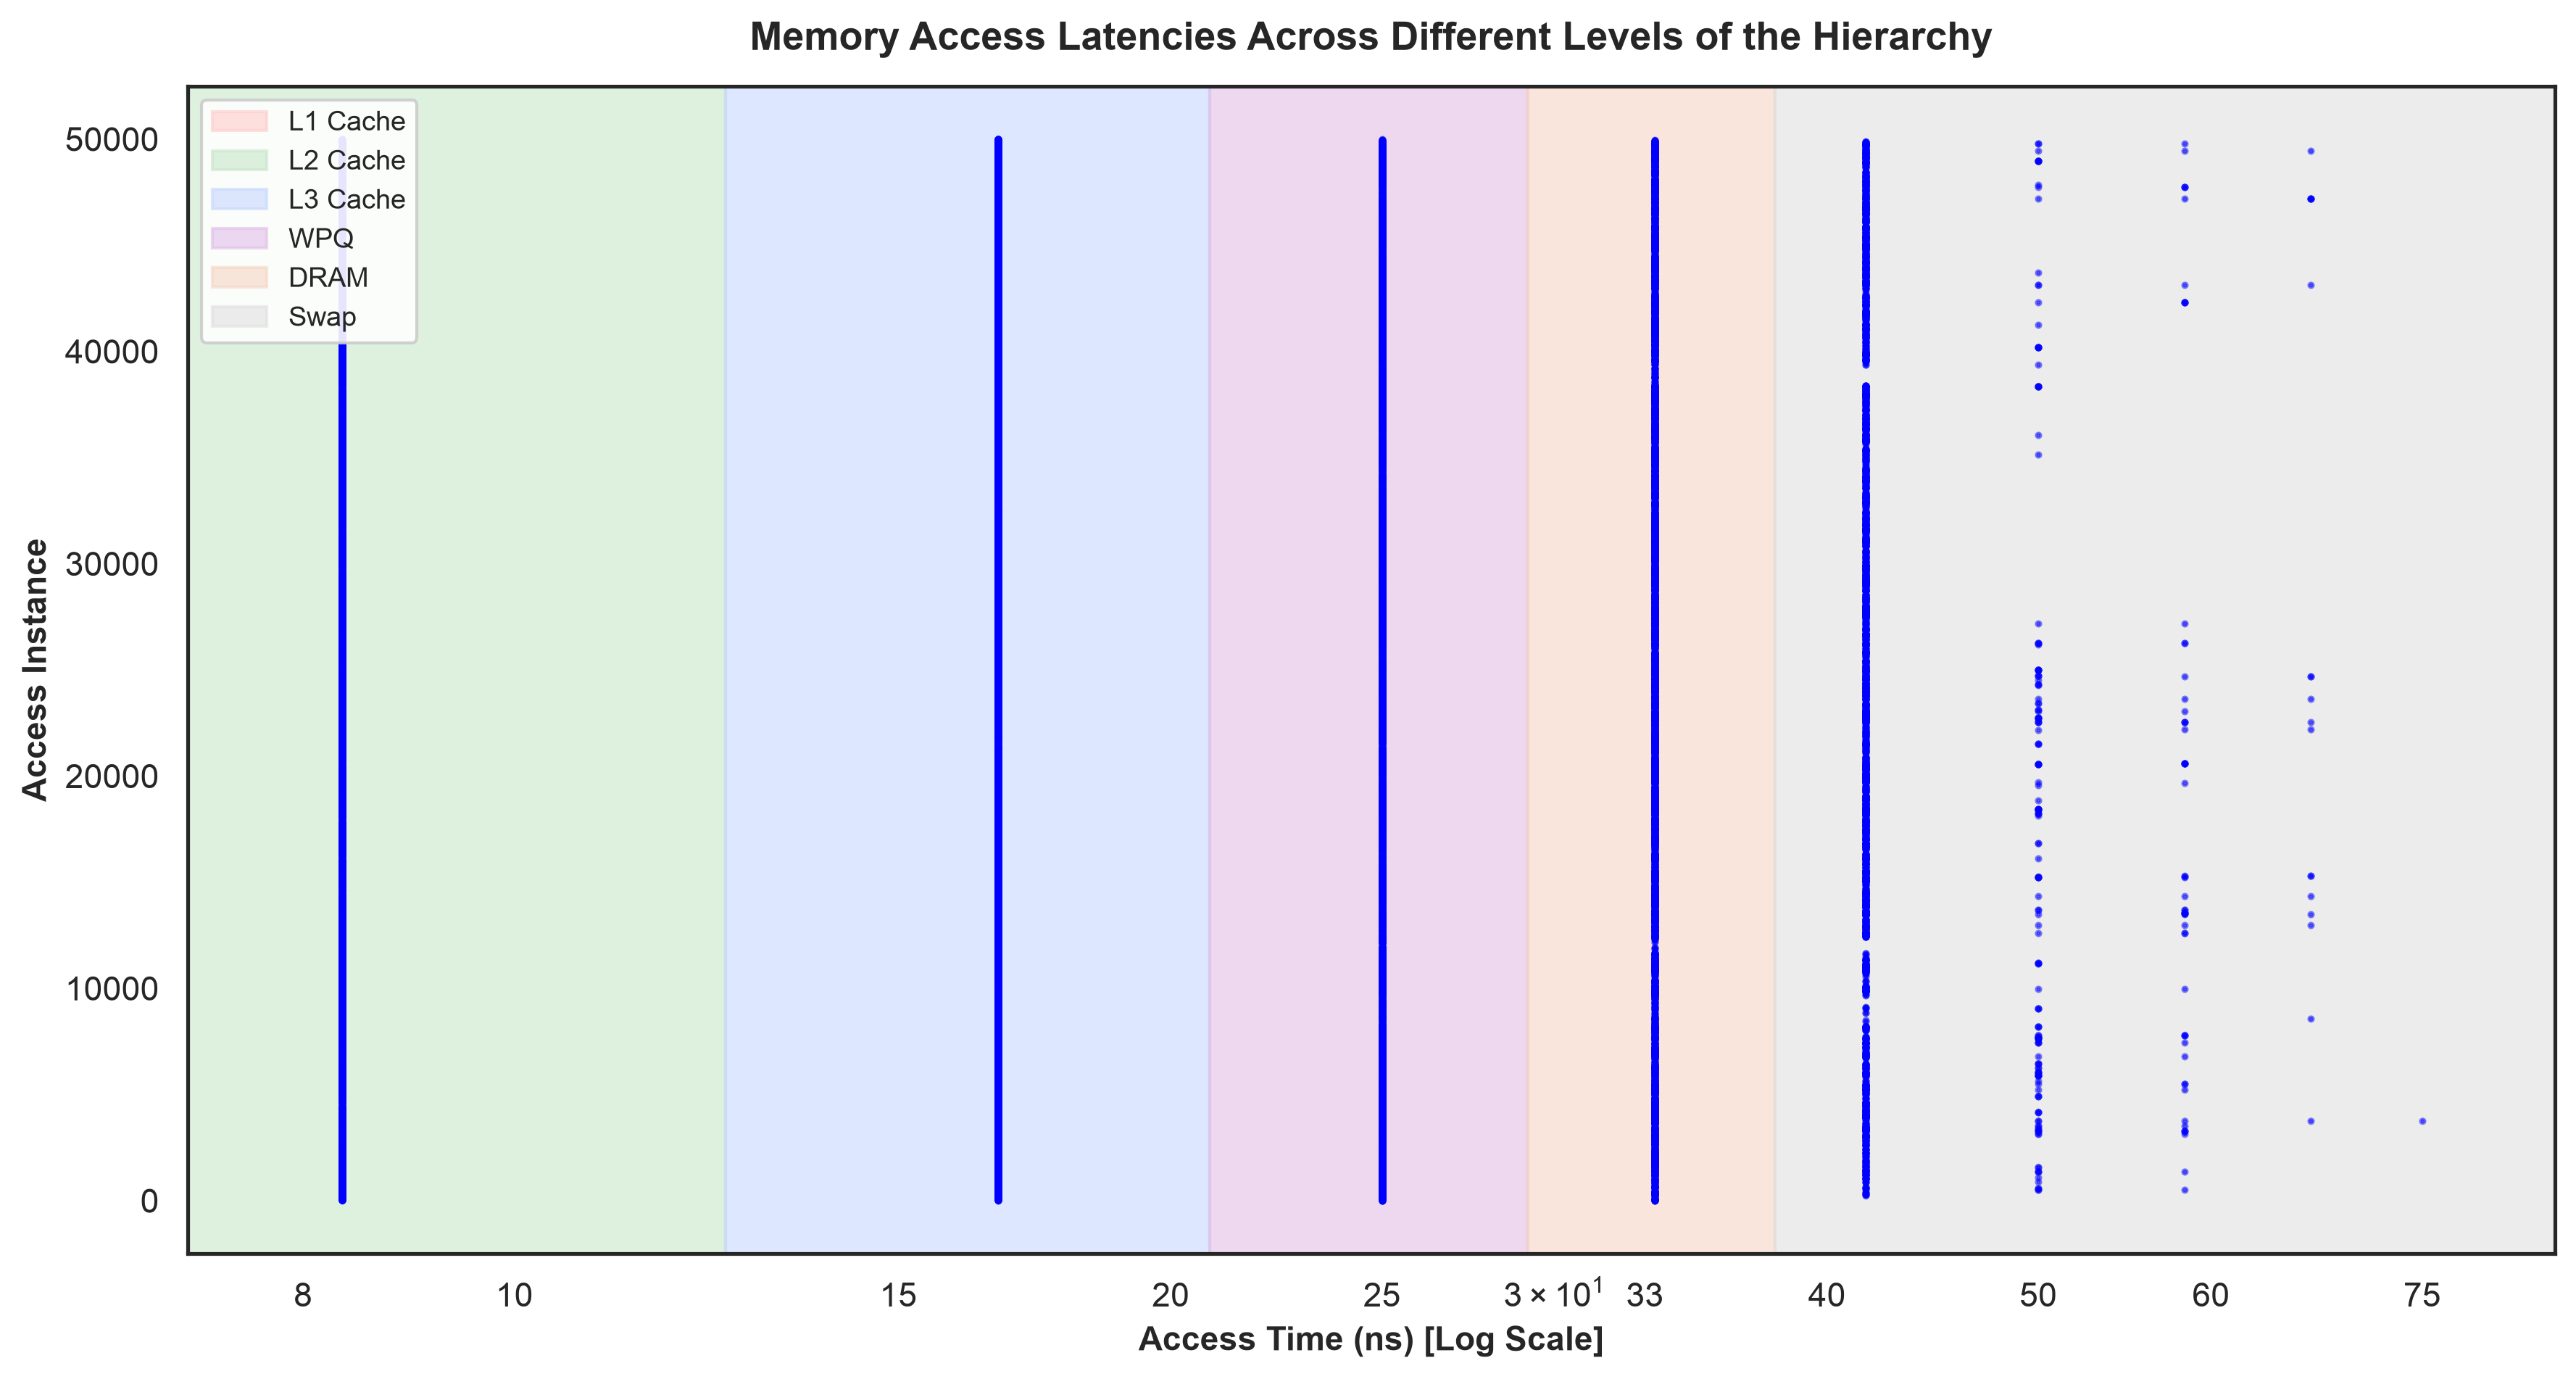
\includegraphics[width=\linewidth]{latency_distribution.png}}
\caption{Empirical memory access latencies categorized by discovered memory hierarchy tiers (log scale). Vertical dashed lines indicate the mean latency for each discovered hardware tier.}
\label{fig:latency}
\end{figure}

\subsection{Analysis of the Measurement Discrepancies}
The pipeline's validation stage compares the discovered clusters against vendor ground truth for the test machine; agreement currently sits at 33.3\% (one of three inferred levels matched within tolerance). This is not a software bug, but a direct reflection of three concrete measurement barriers:

\begin{enumerate}
    \item \textbf{Timer Quantisation:} The data output was highly quantised into discrete steps corresponding to the $\sim$41.7\,ns tick of the Apple Silicon system counter. Because the timer only advances once per tick, measuring a single memory read is physically impossible: the framework was effectively measuring the timer's tick rate rather than memory speed.
    \item \textbf{No User-Space Flush on ARM (mode 1 degenerates):} \texttt{clflush} is an x86-only instruction; it does not exist on ARM, and macOS provides no supported user-space data-cache flush. The probe therefore compiles the flush as a no-op on Apple Silicon, meaning the ``forced DRAM'' mode silently behaves identically to the natural-eviction mode and no deep-memory accesses were ever generated.
    \item \textbf{Write-Before-Read Guarantees L1 Residency:} The most fundamental flaw is in the measurement design itself. To dirty the cache line, the probe writes to the target address immediately before the timed read. That write necessarily pulls the line into L1, so---in the absence of a working flush---every timed read is an L1 hit by construction. Randomising the access pattern does not help here: the probe defeats itself one instruction before each measurement. This, rather than prefetching, is why the L2, L3, and DRAM latencies were completely masked.
\end{enumerate}

A secondary methodological concern was also identified: the moving-average filter smooths across \textit{adjacent samples in collection order}, but since each sample is an independent random access, this blends latencies from different (potential) cache levels together before clustering---actively eroding the step structure the clustering engine is designed to detect. Smoothing is appropriate for a working-set-size sweep curve, not for i.i.d. samples, and will be removed from the sample-based path.

Finally, two reproducibility gaps were noted: the C probe's \texttt{rand()} generator is never seeded, and the Silhouette Score is computed on a 10,000-point subsample without a fixed random state, so successive runs are not exactly repeatable. Both will be fixed with explicit seeds in the final version.

\section{Discussion \& Future Work}
The measurement barriers discovered in initial evaluation provide an excellent foundation for critical analysis and mandate a structural shift in the methodology. The following upgrades will form the core of the final dissertation submission.

\subsection{Working-Set-Size Sweeps with Pointer Chasing}
To eliminate the write-before-read flaw and defeat both the prefetcher and timer quantisation, the C probe will be rewritten around a working-set-size (WSS) sweep with pointer chasing:
\begin{itemize}
    \item For each candidate working-set size, a buffer of that size is initialised as a random cyclic permutation using a Fisher--Yates shuffle \cite{knuth}, and the probe traverses the resulting pointer chain. Each load's address depends on the previous load's result, serialising the accesses and defeating the prefetcher without any explicit flush---sizes larger than a given cache level naturally overflow it.
    \item To bypass the coarse timer, the probe will execute on the order of $10^4$ dependent hops inside a single timing window and divide the elapsed time by the hop count, achieving sub-nanosecond effective precision via batch amortisation.
\end{itemize}

\subsection{Robust Boundary Extraction}
The current extraction method relies on the absolute minimum and maximum of each cluster. As noted by Klimis et al. \cite{klimis2025}, micro-architectural noise makes this fragile: a single slow L1 access mis-clustered as ``L2'' drags the boundary upward. The future implementation will use the 5th and 95th percentiles and a sliding-window majority vote to compute boundaries that are robust to such outliers.

\subsection{Change-Point Detection}
K-Means fundamentally assumes compact, roughly spherical clusters, but latency-versus-WSS data forms a step function blurred by prefetchers and TLB misses. The machine learning engine will therefore be extended with change-point detection algorithms (via the \texttt{ruptures} library \cite{ruptures}), which are mathematically designed to identify the exact points at which a flat latency curve suddenly shifts, and the two approaches will be compared empirically.

\section{Conclusion}
The initial development of the Auto-Echo framework has successfully established the core infrastructure required to capture low-level memory timings and automatically process them through an unsupervised machine learning pipeline. Crucially, empirical testing exposed exactly where the naive measurement design fails on modern hardware: a timer whose tick dwarfs an L1 hit, the absence of a user-space flush on ARM, and a write-before-read pattern that guaranteed L1 residency of every measured access. By pivoting to a batch-amortised, pointer-chasing WSS methodology with robust percentile boundaries and change-point detection, the final project is well positioned to achieve accurate, architecture-agnostic memory echolocation.

\begin{thebibliography}{00}
\bibitem{klimis2025} V. Klimis et al., ``Shouting at memory: Where did my write go?'' in \textit{Proc. 39th European Conf. on Object-Oriented Programming (ECOOP)}, 2025.
\bibitem{apple_mach} Apple Inc., ``mach\_absolute\_time -- Apple developer documentation,'' 2024. [Online]. Available: https://developer.apple.com/documentation/kernel/1462446-mach\_absolute\_time
\bibitem{lof} M. M. Breunig, H.-P. Kriegel, R. T. Ng, and J. Sander, ``LOF: Identifying density-based local outliers,'' in \textit{Proc. ACM SIGMOD Int. Conf. on Management of Data}, 2000, pp. 93--104.
\bibitem{silhouette} P. J. Rousseeuw, ``Silhouettes: A graphical aid to the interpretation and validation of cluster analysis,'' \textit{J. Comput. Appl. Math.}, vol. 20, pp. 53--65, 1987.
\bibitem{knuth} D. E. Knuth, \textit{The Art of Computer Programming, Vol. 2: Seminumerical Algorithms}, 3rd ed. Reading, MA: Addison-Wesley, 1997.
\bibitem{ruptures} C. Truong, L. Oudre, and N. Vayatis, ``Selective review of offline change point detection methods,'' \textit{Signal Processing}, vol. 167, 107299, 2020.
\bibitem{scikit-learn} F. Pedregosa et al., ``Scikit-learn: Machine learning in Python,'' \textit{J. Mach. Learn. Res.}, vol. 12, pp. 2825--2830, 2011.
\end{thebibliography}

\end{document}
